\chapter{Differential Privacy in Machine Learning}

Machine learning models can also be regarded as queries on a data set. A DP mechanism can be applied to them at different points in time, as can be seen in \autoref{fig:design_principles_dpml}. Adding noise in the respective steps has various advantages and disadvantages.

\begin{figure}[tb]
  \centering
  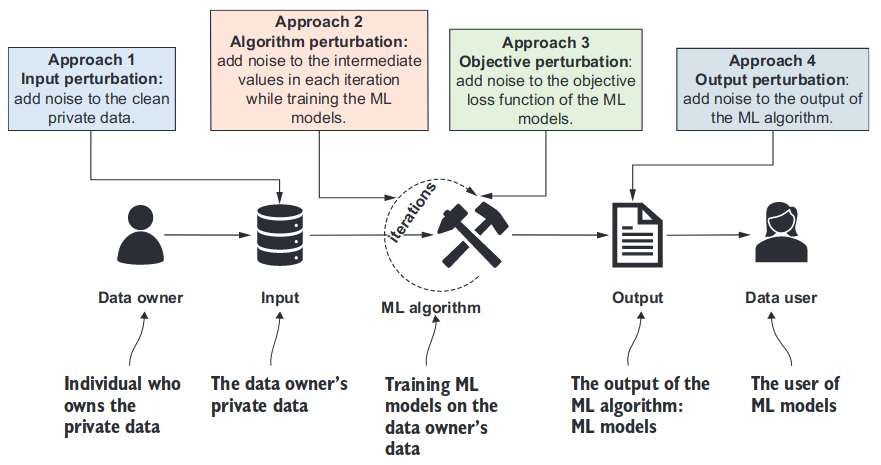
\includegraphics[width=0.7\textwidth]{Bilder/design_principles_dpml.png}
  \caption{Design principles of differentially private ML from \textcite{chang:2023}}
  \label{fig:design_principles_dpml}
\end{figure}

With \textit{input pertubation}, noise is added to the training data before training. This is easy to implement and versatile, but also requires a larger amount of noise as the data usually has a high \textit{sensitivity}.

Using \textit{algorithm pertubation}, the models are trained with unchanged data. In iterative algorithms, the intermediate results can be distorted in the individual steps. \textcite{abadi:2016}, for example, add noise to the gradients.

\textit{Output pertubation} adds noise to the outputs generated by the model. However, the method is not applicable if the model is to be published, as the number of requests to the model cannot be predicted and therefore no privacy guarantees are possible.

With \textit{Objective pertubation}, noise is added to the \textit{Objective function} for which the model is optimised.

The Differentially Private-Stochastic Gradient Descent (DP-SGD) presented by \textcite{abadi:2016} is now a widely used algorithm for training neural networks, on which many other works are based. It is based on the \textit{Stochastic Gradient Descent} (SGD), an iterative optimisation algorithm that is used in various machine learning methods. Compared to the SGD, the DP-SGD has some additional hyperparameters to fulfil the privacy guarantees:

\begin{itemize}
  \item \textbf{Noise scale $\sigma$} A factor by which the noise of the DP mechanism is controlled. 
  \item \textbf{Lot size $L$} The number of data points that are included in a gradient update.
  \item \textbf{Gradient norm bound $C$} All calculated gradients are clipped so that they have a maximum $\ell_2$ norm of $C$. This is necessary because noise with the Gaussian mechanism is added in the following and the sensitivity of vectors is defined via the $\ell_2$ norm. 
\end{itemize}

During training, these parameters affect how quickly a desired $(\epsilon, \delta)$ privacy budget is exhausted. In their results, \textcite{abadi:2016} show that the choice of these parameters (in addition to the parameters from the normal SGD) also has an effect on the accuracy of the model under a fixed privacy budget.

In addition to the specific algorithm, \textcite{abadi:2016} developed the \textit{Moments Accountant}, a method for estimating the loss of privacy during training, which is asympotically much more accurate than classical estimates using composition theorems. They prove this benefit in their work through empirical experiments.

In their paper, \textcite{mcmahan:2018} develop a variant of the \textit{Federated Averaging} (FedAvg) algorithm \parencite{mcmahan:2016} based on the work of \textcite{abadi:2016}, which ensures DP guarantees for users. Their goal is to train an LSTM model for \textit{Next-Word Prediction} on mobile devices. They transfer the definition of adjacent datasets to federated learning by defining the neighbourhood by adding or removing all data of a user. In their experiments, they show that the accuracy of the model can be maintained under DP guarantees, but at a higher computational cost.

The main changes compared to the non-private FedAvg are a limited sensitivity at the clients (by clipping) and at the server (by estimators of the aggregation with a limited range of values). In addition, the server adds noise to the aggregated update based on sensitivity.

\section{Differential privacy with heterogeneous privacy budgets}

\textcite{boenisch:2023} show that the assumption of a privacy budget for all data points limits the possibilities of a model to learn from a data set, since the strictest privacy budget must be assumed for all. In reality, however, different users who generate the data have different privacy requirements. They provide two approaches for training with heterogeneous privacy budgets: the first (\textbf{SAMPLE}) utilises the privacy budget of less private data points by drawing them with a higher probability during training. The second approach (\textbf{SCALE}) controls the privacy budget used by individualising the \textit{noise multiplier} and \textit{clipping norms}.

\textcite{aldaghri:2023} present an algorithm to benefit from heterogeneous privacy requirements in federated learning scenarios. Similar to the \textbf{SCALE} algorithm from \textcite{boenisch:2023}, it uses individual noise scales for each group with the same privacy level. In addition, only two gradations of privacy levels are evaluated, namely clients without privacy requirements and clients with privacy requirements. To track the \textit{privacy loss} they use a moments accountant from \textcite{abadi:2016} for each group of cleints with the same privacy requirements.

